\documentclass{homework}

\title{Homework 8}
\author{Kevin Evans}
\studentid{11571810}
\date{March 25, 2020}
\setclass{Physics}{304}
\usepackage{amssymb}
\usepackage{mathtools}

\usepackage{amsthm}
\usepackage{amsmath}
\usepackage{slashed}
\usepackage{relsize}
\usepackage{threeparttable}
\usepackage{float}
\usepackage{booktabs}
\usepackage{boldline}
\usepackage{changepage}
\usepackage{physics}
\usepackage[inter-unit-product =\cdot]{siunitx}
\usepackage{setspace}

\usepackage[makeroom]{cancel}
\usepackage{pgfplots}

\usepackage{multicol}
\usepackage{tcolorbox}
\usepackage{enumitem}
\usepackage{times}
\usepackage{mhchem}
\usepackage{graphicx} 
\DeclareSIUnit{\year}{yr}

\begin{document}
	\maketitle
	\subsubsection*{Chapter 11}
	\begin{enumerate}[label={\arabic*.}]
		\item \begin{itemize}
			\item Ionic bonds are formed when one or more electrons is transferred between two oppositely-charged ions, such as sodium chloride (\ce{Na+}, \ce{Cl-}).
			\item Covalent bonds are created when electrons are shared between two atoms, such as molecular oxygen (\ce{O=O}) or the triple-bond in ethyne (\ce{H-C#C-H}).
			\item van der Waals bonds occur due to electrostatic forces and are between molecules, unlike the intramolecular ionic and covalent bonding. \begin{itemize}
				\item Dipole-dipole forces are forces due to the attraction between molecules with permanent dipoles.
				\item Dipole-induced forces are essentially the same as the dipole-dipole forces, but one of the molecules is non-polar and the polar molecule induces a dipole moment.
				\item The dispersion force occurs between two non-polar molecules but random fluctuations can induce a temporary dipole, leading to an electrostatic electric force.
			\end{itemize}
			\item Hydrogen bonding occurs both at an inter- and intramolecular level, between hydrogen and a selection of other elements (F, O, N).
		\end{itemize}
		\item \begin{enumerate}
			\item Since \ce{Kr} has a full octet, it'll only form \textbf{van der Waals bonds}.
			\item \textbf{Ionic bonds}, as \ce{K+} and \ce{Cl-} can exchange an atom to become a neutral molecule.
			\item \textbf{Hydrogen bond}, since fluorine H-bonds.
		\end{enumerate}
	
		\item \begin{enumerate}
			\item For the Lennard-Jones potential of \begin{align*}
			U(r) & = \frac{A}{r^{12}} - \frac{B}{r^6}
			\intertext{The minimum distance is given by equating the first derivative to zero,}
			\dv{U}{r} & = -12A r^{-13} + 6Br^{-7} = 0 \\
			0 & = -\frac{6\left(2A - Br^6\right)}{r^{13}}
			\intertext{The trivial root is given by the $r^{13}$ bit and is noting the stability at $r\to \infty$. The nontrivial root is the stable distance $r_0$,}
			0 & = 2A - Br^6 \\
			r_0 & = \left(\frac{2A}{B}\right)^{1/6}
			\end{align*}
		\item If the diatomic particle obeys the potential above, it'd be difference in energy between $r=r_0$ and $r \to \infty$. \begin{align*}
			U(r_0) & = \frac{A}{\left[ \left(2A/B\right)^{1/6} \right]^{12}} - \frac{B}{ \left[\left(2A/B\right)^{1/6}\right]^6} \\
				& = \frac{B^2}{4A} - \frac{B^2}{2A} \\
				& = -\frac{B^2}{4A}
			\intertext{At $r\to\infty$, the potential energy is $0$. So the energy required is}
			E & = \frac{B^2}{4A}
		\end{align*}
		\end{enumerate} 
	
	
		\item It's non-directional since the electrostatic forces have an equal force for any charge in any direction--there's no inherit direction in the electric forces.
		
		\item Translational motion of the entire molecule, rotational energy about axes perpendicular to the molecular axis, and vibrational energy between the two atoms. Probably the translational is easiest to excite. The vibrational mode is the most difficult to excite (described in Problem 8).
		
		\item The first term $\left(v + \frac{1}{2}\right)\hbar \omega$ comes from the vibrational energy and is the same as a one-dimensional oscillator. It has parameters of the vibrational quantum number $v$ and frequency $\omega$.
		
		The second term $\dfrac{\hbar^2 \ell (\ell + 1)}{2 I_{CM}}$ relates to the rotational energy of both atoms in the diatomic molecule. The energy is parameterized by the rotational quantum number $\ell$ and moment of inertia $I_{CM}$ (about the CM of the two atoms).
		
		\item For vibrational energy, the frequency is related to the reduced mass as $\omega \propto 1/\sqrt{\mu}$. If the mass is doubled, the reduced mass would be doubled as well. The vibrational energy of \ce{D_2} is less than \ce{H_2} as
		\[E_{v\ce{D_2}} \approx 0.707 \times E_{v\ce{H_2}}\]
		
		For the rotational energy, the moment of inertia is proportional to the reduced mass. As the mass is doubled, the inertia is doubled, so the rotational energy is doubled as well,
		\[E_{l\ce{D_2}} = 2 \times E_{l\ce{H_2}}\]
		
		\item Rotational requires less energy. If we take the values for the first transition ($0 \to 1$) of \ce{CO}, the rotational transition has a frequency of \SI{1.15e11}{\Hz}, which is much lower than the vibrational transition with \SI{6.42e13}{\Hz}.
		
		\pagebreak
		\item For $\Delta v = 1$, the change in vibrational energy is $\Delta E_v = \hbar \omega_0$, as the $\frac{1}{2}$ term cancels.
		
		For $\Delta \ell = \ell_f - \ell_i = +1$: \begin{align*}
			E_\mathrm{phot} & = \hbar \omega_0 + \frac{\hbar^2 \ell_f(\ell_f + 1)}{2 I_{CM}}
			- \frac{\hbar^2 \ell_i(\ell_i + 1)}{2 I_{CM}}
			\intertext{But as $\ell_i + 1 = \ell_f$, we can substitute it in the last term,}
			E_\mathrm{phot} & = \hbar \omega_0 + \frac{\hbar^2 \ell_f(\ell_f + 1)}{2 I_{CM}}
- \frac{\hbar^2 \ell_f(\ell_f - 1)}{2 I_{CM}}
			\intertext{Evaluating this, the $\ell_f^2$ terms cancel and the $2/2$ bits cancel,}
			E_\mathrm{phot} & = \hbar \omega_0 + \frac{\hbar^2 \ell_f}{I_{CM}} \qed
		\end{align*}
	
		For $\Delta \ell = \ell_f - \ell_i = -1$: \begin{align*}
			E_\mathrm{phot} & = \hbar \omega_0 + \frac{\hbar^2 \ell_f(\ell_f + 1)}{2 I_{CM}}
			- \frac{\hbar^2 \ell_i(\ell_i + 1)}{2 I_{CM}} \\
			& = \hbar \omega_0 + \frac{\hbar^2 (\ell_i - 1)(\ell_i - 1 + 1)}{2 I_{CM}}
				- \frac{\hbar^2 \ell_i(\ell_i + 1)}{2 I_{CM}} \\
			& = \hbar \omega_0 + \frac{\hbar^2 \ell_i (\ell_i - 1)}{2 I_{CM}}
			- \frac{\hbar^2 \ell_i(\ell_i + 1)}{2 I_{CM}}
		\intertext{The $\ell_i^2$ terms cancel and we're left with $-2 \times \ell_i$,}
		E_\mathrm{phot} & = \hbar \omega_0 - \frac{\hbar^2}{I_{CM}} \ell_i \qed
		\end{align*}
	
		\item For the LHS of the energy level diagram, $\Delta \ell = +1$. The RHS shows $\Delta \ell = -1$. So, it'd be likely symmetric and centered about the frequency $\omega_0$,

		\begin{center}
			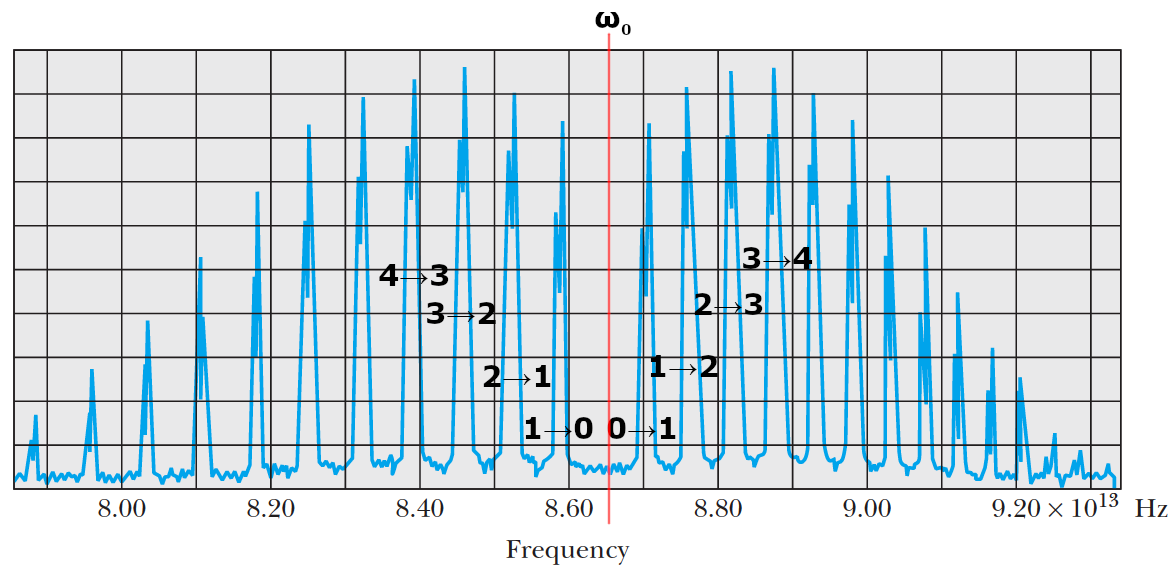
\includegraphics[width=\linewidth]{screenshot001}
		\end{center}
		
	\end{enumerate}
\end{document}